\documentclass[xcolor={svgnames}]{beamer}

\setbeameroption{hide notes} 

%\usetheme{NLP}
\usepackage{beamerthemesplit}
\usetheme{default}
\useoutertheme{infolines}

\usepackage{graphicx}
\usepackage{lmodern}

\usepackage{soul}

\usepackage{amsmath,amsthm,amssymb}   

\usepackage{listings}

\usepackage{algorithm,algorithmic}

\usepackage{tikz}
\usetikzlibrary{positioning,shapes,shadows,arrows}

% Text
\newcommand{\todo}[1]{\hl{\textbf{TODO:} #1}}
\newcommand{\citationneeded} {\ensuremath{^{[\textrm{citation needed}]}}}


%Math Operators
%\DeclareMathOperator {\argmax} {argmax}
%\DeclareMathOperator {\argmin} {argmin}
\DeclareMathOperator {\sgn} {sgn}
\DeclareMathOperator {\trace} {tr}
\DeclareMathOperator{\E} {\mathbb{E}}
\DeclareMathOperator{\Var} {Var}
\DeclareMathOperator{\diag} {diag}
\DeclareMathOperator{\triu} {triu}
\DeclareMathOperator{\mult} {Multinomial}
\DeclareMathOperator{\normalt} {Normal}
\DeclareMathOperator{\cvec} {cvec}

\newcommand{\ud}{\, \mathrm{d}}
\newcommand{\diff}[1] {\frac{\partial}{\, \partial #1}}
\newcommand{\difff}[2] {\frac{\partial^2}{\, \partial #1\, \partial #2}}
\newcommand{\diffn}[2] {\frac{\partial^{#2}}{\, \partial {#1}^{#2}}}
\newcommand{\tuple}[1] {\langle #1 \rangle}
\newcommand{\innerprod}[2] {\langle #1, #2 \rangle}

% Constants/etc.
\renewcommand{\Re} {\mathbb{R}}
\newcommand{\Cm} {\mathbb{C}}
\newcommand{\Qm} {\mathbb{Q}}
\newcommand{\half} {\frac{1}{2}}

\newcommand{\inv}[1] {{#1}^{-1}}

\newcommand{\normal}[2] {\mathcal{N}(#1, #2)}
\newcommand{\mL} {\mathcal{L}}

\newcommand\eqdef{\ensuremath{\stackrel{\rm def}{=}}} % Equal by definition
\newcommand\refeqn[1]{(\ref{eqn:#1})}
\newcommand\sD{\ensuremath{\mathcal{D}}}
\newcommand\sM{\ensuremath{\mathcal{M}}}
\newcommand\refapp[1]{Appendix~\ref{sec:#1}}
\newcommand\refthm[1]{Theorem~\ref{thm:#1}}
\newcommand\sigmamin{\sigma_\text{\rm min}}
\newcommand\sigmamax{\sigma_\text{\rm max}}
\newcommand\op{{\text{\rm op}}}
\newcommand\BP{\ensuremath{\mathbb{P}}}
\newcommand\reflem[1]{Lemma~\ref{lem:#1}}

\newcommand{\sidenote}[1]{\begin{itemize} \item #1 \end{itemize}}
\newcommand{\hlmath}[1]{\textrm{\color{blue}\ensuremath{#1}}}

\pgfdeclarelayer{bg}
\pgfsetlayers{bg,main}
\newcommand{\obj}[1]{%
    {%
    \begin{minipage}{6cm}
      #1
    \end{minipage}
    }
}
\newcommand{\objw}[2]{%
    {%
    \begin{minipage}{#1}
      #2
    \end{minipage}
    }
}
\tikzstyle{box}=[scale=0.8,rectangle,fill=white,draw=black]
\tikzstyle{loop}=[smooth,dashed,in=-90,out=-90,looseness=0.75]

\makeatletter
\newcommand*{\centerfloat}{%
  \parindent \z@
  \leftskip \z@ \@plus 1fil \@minus \textwidth
  \rightskip\leftskip
  \parfillskip \z@skip}
\makeatother

% Tensor powers
\newcommand{\tp}[1] {^{\otimes #1}}

% Matrix Perturbation
\newcommand{\pinv}[1] {#1^{\dagger}}
\newcommand{\Ap} {\hat{A}}
\newcommand{\Bp} {\hat{B}}
\newcommand{\Up} {\hat{U}}
\newcommand{\Vp} {\hat{V}}
\newcommand{\Xp} {\hat{X}}
\newcommand{\Wp} {\hat{W}}
\newcommand{\cM} {\mathcal{M}}
\newcommand{\cMp} {\hat{\mathcal{M}}}
\newcommand{\Mp} {\hat{M}}
\newcommand{\Zp} {\hat{Z}}
\newcommand{\vp} {\hat{v}}
\newcommand{\lambdap} {\hat{\lambda}}
\newcommand{\sigmap} {\hat{\sigma}}
\newcommand{\mup} {\hat{\mu}}
\newcommand{\cnd}[1] {\kappa(#1)}
\newcommand{\aerr}[1] {\varepsilon_{#1}}
\newcommand{\rerr}[1] {\delta_{#1}}
\newcommand{\serr}[1] {\alpha_{#1}}
\newcommand{\berr}[1] {\beta_{#1}}
\newcommand{\gap}[1] {\Delta_{#1}}

% Keywords
\newcommand{\Pairs}{\mathrm{Pairs}}
\newcommand{\Triples}{\mathrm{Triples}}



% these will be used later in the title page
\title[Spectral Experts]{Spectral Experts for Estimating Mixtures of Linear Regressions}
\author[Chaganty, Liang]{%
    Arun Tejasvi Chaganty\\
    Percy Liang
}
\institute{Stanford University}

\begin{document}

% "Beamer, do the following at the start of every section"
\AtBeginSection[] 
{%
\begin{frame}<beamer> 
\frametitle{Outline} % make a frame titled "Outline"
\tableofcontents[currentsection]  % show TOC and highlight current section
\end{frame}
}

\begin{frame}
  \titlepage
\end{frame}

\begin{frame}
  \frametitle{Generative vs. Discriminative Latent Variable Models}

  \begin{tikzpicture}
    % Tasks.
    \node[style=box] (gen) at (0,0) {\objw{6cm}{%
      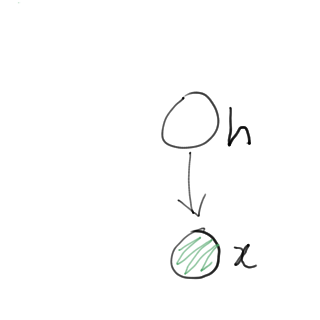
\includegraphics[width=\textwidth,height=3cm,keepaspectratio]{figures/gen.png}\\
      \hfill Generative Models
      }};
    \node[scale=0.7] at (0.5,0.5) {Latent variable};

    \node<2->[style=box,below=0.1cm of gen] {\obj{%
      {\bf Generative Models}
      \begin{itemize}
        \item Gaussian Mixture Models
        \item Hidden Markov Models
        \item Latent Dirichlet Allocation
        \item PCFGs
        \item \dots
      \end{itemize}
      }};
    \node<3->[style=box] (disc) at (6,0) {\objw{6cm}{%
      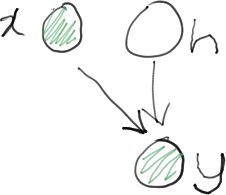
\includegraphics[width=\textwidth,height=3cm,keepaspectratio]{figures/disc.png}\\
      \hfill Discriminative Models
      }};
    \node<4->[style=box,below=0.1cm of disc] (disc-models) {\obj{%
    {\bf Discriminative Models}
      \begin{itemize}
        \item Logistic Regression
        \item Latent CRFs
        \item Discriminative LDA
        %\item Semi-Latent Topic Models (Wang and Mori, 2009)
        %\item Discriminative Parsers (Liang et.\ al, 2006)
        \item \dots
      \end{itemize}
      }};
    \node<5->[style=box,below=0.1cm of disc-models] {\obj{%
      {\bf Easy to include features and tend to be more accurate.}
    }};

  \end{tikzpicture}

  % Really do known Gen (HMMs, ) vs Disc (CRFs) models 

    \note[item]{Would like to start by talking about the bigger picture of parameter estimation.}
    \note[item]{Discriminative Latent Variable Models are useful, but hard to learn.}
    \note[item]{Split models into generative and discriminative models.}
    \note[item]{Discriminative LVMs combine the predictive accuracy with compact expressiveness.}
    \note[item]{They have been used in several applications, e.g.\ object recognition, syntactic parsing, machine translation, etc.}
    \note[item]{Learning parameters for these models is hard because they have non-convex likelihood functions.}
\end{frame}

\begin{frame}
  \frametitle{Parameter Estimation is Hard}

  \begin{tikzpicture}
    % x, y
    \node[style=box] at (0,-1.5) {\objw{12cm}{%
    \includegraphics<1>[width=\textwidth,height=6cm,keepaspectratio]{figures/likelihood.png}
    \includegraphics<2>[width=\textwidth,height=6cm,keepaspectratio]{figures/likelihood-mle.png}
    \includegraphics<3>[width=\textwidth,height=6cm,keepaspectratio]{figures/likelihood-em.png}
    \includegraphics<4>[width=\textwidth,height=6cm,keepaspectratio]{figures/likelihood-mom.png}
      \hfill{\em expected log-likelihood}
      }};
  \end{tikzpicture}

  % Simple message: MLE is consistent but intractable, EM is efficient not but consistent. Can we get something in between.

  \begin{itemize}
    \item<1-> Log-likelihood function is non-convex.
    \item<2-> MLE is consistent but intractable.
    \item<3-> EM is efficient but inconsistent.
    \item<4-> Can we build {\bf efficient yet consistent estimators} that get better with more data?
  \end{itemize}

  \note[item]{We would like to develop efficient consistent estimators for discriminative LVMS.}
  \note[item]{Past approaches rely on local optimization, which are susceptible to local optima.}
  \note[item]{And they don't just go away with more data.}
  \note[item]{Recently, there has been work on consistent parameter
      estimation for generative LVMS\@. We'd like to extend their work to
      the discriminative case.}
\end{frame}

\begin{frame}
  \frametitle{Method of Moments a.k.a.\ Spectral Methods}
  \begin{itemize}
    \item<+-> Method of Moments [Pearson, 1894]
    \item<+-> Observable operator models
    \begin{itemize}
      \item Subspace identification [Ljung, 1987]
      \item Observable operator models [Jaeger, 2000]
        \note[item]{Entry point into machine learning}
      \item {\bf Hidden Markov models [Hsu et al, 2009]}
        \note[item]{Entry point into machine learning}
      \item Low-treewidth graphs [Parikh et al., 2012]
      \item Weighted finite state automata [Balle \& Mohri, 2012]
    \end{itemize}
     \item<+-> Parameter Estimation
  \begin{itemize}
    \item Mixture of Gaussians [Kalai/Moitra/Valiant, 2010]
    \item {\bf Mixture models, HMMs [Anandkumar/Hsu/Kakade, 2012]}
    \item Latent Dirichlet Allocation [Anandkumar/Hsu/Kakade, 2012]
    \item Stochastic block models [Anandkumar/Ge/Hsu/Kakade, 2012]
    \item Linear Bayesian networks [Anandkumar/Hsu/Javanmard/Kakade, 2012]
  \end{itemize}
  \end{itemize}
\end{frame}

\begin{frame}
  \frametitle{Example: Gaussian Mixture Model}
  \begin{tikzpicture}
    % x, y
    \node<1->[style=box] (defn) at (0,0) {\objw{6cm}{%
    \begin{itemize} 
      \item Generative process:
      \begin{align*}
        h \in [k] &\sim \Mult(\pi) \\
        x &\sim \normal{\beta_h}{\sigma^2}.
      \end{align*}
    \end{itemize}
    }};
    \node<1->[style=box] (models) at (6,0) {\objw{6cm}{%
      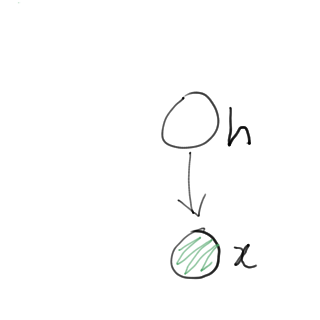
\includegraphics[width=0.45\textwidth,height=3cm,keepaspectratio]{figures/gen.png}
      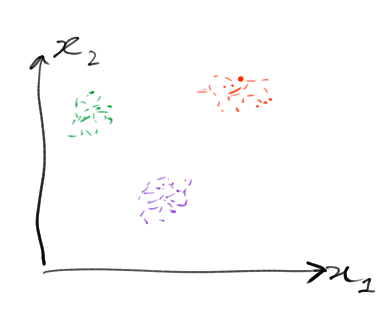
\includegraphics[width=0.45\textwidth,height=3cm,keepaspectratio]{figures/mog.png}
    }};

    \node<2->[style=box,below=0.1cm of defn] {\objw{6cm}{%
    \begin{itemize} 
      \item Moments:
    \begin{align*}
        \action<2->{%
        \E[x|h] &= \beta_h \\
        }
        \action<3->{%
        \E[x] &= \sum_h \pi_h \beta_h \\
        }
        \action<4->{%
        \E[x\tp{2}] &= \sum_h \pi_h \beta_h{\hlmath{\tp{2}}} \\
                    &= \sum_h \pi_h (\beta_h \beta_h^T) \\
                    }
        \action<5->{%
        \E[x\tp{3}] &= \sum_h \pi_h \beta_h\tp{3}.
        }
      \end{align*}
    \end{itemize}
    }};
    %\tikzrect{1}{1};
    \uncover<4->{%
    \tikzrect{black,fill=white}{(6,-2)}{1}{1};
    \node at (7,-2.5) {$\E[x\tp{2}]$};
    \node at (4.5,-2.5) {$d$};
    }
    \uncover<5->{%
    \tikzcube{black,fill=white}{(6,-4,0)}{1}{1}{1};
    \node at (7,-4.5,0) {$\E[x\tp{3}]$};
    \node at (4.5,-4.5) {$d$};
    \node at (4.5,-4.5) {$d$};
    }
  \end{tikzpicture}

\end{frame}

\begin{frame}
  \frametitle{Aside: Tensor Operations}
  \begin{tikzpicture}
    % x, y
    \node<1->[style=box] (defn) at (0,0) {\objw{6cm}{%
    \begin{align*}
        \action<1->{%
        x\tp{3}_{ijk} &= x_i x_j x_k \comment{indexing}\\
        }
        \action<2->{%
        A \cdot B &= \sum_{ijk} A_{ijk} B_{ijk} \comment{inner product}\\
        }
        \action<3->{%
        A(u)_{ij} &= \sum_{k} A_{ijk} u_k \comment{projection}\\
        }
        \action<4->{%
        A(u,v)_{i} &= \sum_{jk} A_{ijk} u_j v_k \comment{projection} \\
        }
      \end{align*}
    }};
    \tikzcube{black,fill=white}{(6,2,0)}{1}{1}{1};
    \node (pt) at (5.75,1.75,0) {$\hlmath{\times}$};
    \uncover<3->{%
    \tikzrect{black,fill=white}{(6,0)}{1}{1};
    }
    \uncover<4->{%
    \tikzrect{black,fill=white}{(6,-2)}{0.1}{1};
    }
  \end{tikzpicture}

\end{frame}


\begin{frame}
  \frametitle{Example: Gaussian Mixture Model}
  \begin{tikzpicture}
    % x, y
    \node<1->[style=box] (moments) at (0,0) {\objw{6cm}{%
      Assume $\beta_h$ to be orthogonal;
      \begin{align*}
        \E[x\tp{3}] &= \sum_{h=1}^k \pi_h \beta_h\tp{3}. 
      \end{align*}
    }};
    \node<1->[style=box] (models) at (6,0) {\objw{6cm}{%
      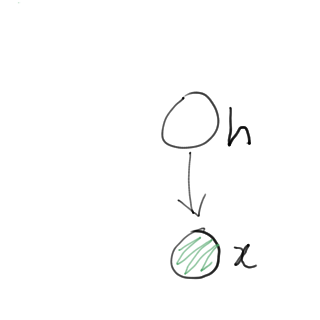
\includegraphics[width=0.45\textwidth,height=3cm,keepaspectratio]{figures/gen.png}
      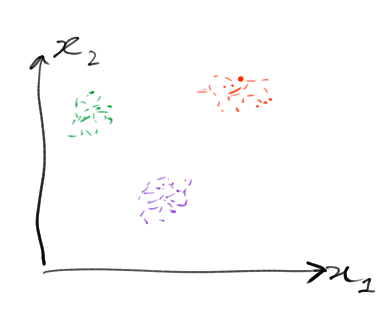
\includegraphics[width=0.45\textwidth,height=3cm,keepaspectratio]{figures/mog.png}
    }};

    \node<1-> at (0,-3) {\objw{6cm}{%
    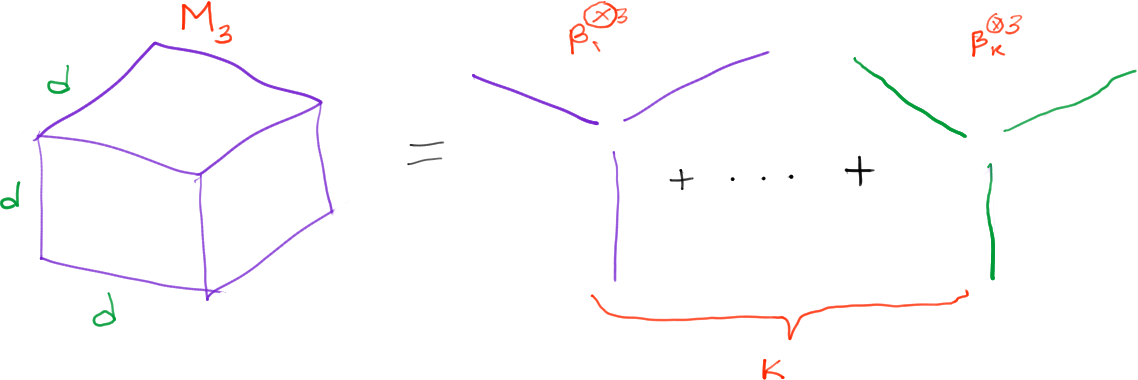
\includegraphics[width=\textwidth,height=6cm,keepaspectratio]{figures/tensor.png}
      }};
    \node<2->[style=box] at (6,-3) {\objw{6cm}{%
      $\beta_h$ are eigenvectors!
        \begin{align*}
          \E[x\tp{3}](\beta_h,\beta_h) 
            %&= \sum_{h'=1}^k \pi_{h'} (\beta_{h}^T \beta_{h'})^2 \beta_{h'} \\
            %&= \sum_{h'=1}^k \pi_{h'} \delta_{hh'} \beta_{h'} \\
            &= \pi_{h} \beta_{h}.
        \end{align*}

        \hfill{\em Anandkumar, Hsu, et.\ al (2012)}
      }};
%
%    \node<2>[style=box,below=0.1cm of tensorf] {\objw{12cm}{%
%    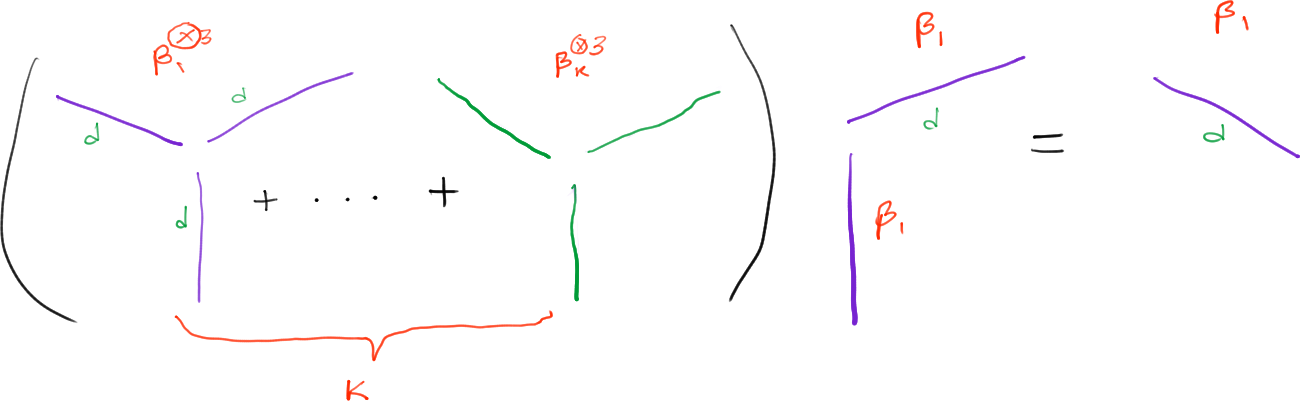
\includegraphics[width=\textwidth,height=6cm,keepaspectratio]{figures/tensor-decomp.png}
%      \hfill {Tensor Power Method}
%      }};
  \end{tikzpicture}

    \note[item]{\bf We can recover the means of a generative LVM by exploiting their symmetric structure.}
    \note[item]{\begin{align*} M_2 &= \sum_{h=1}^k \pi_h \beta_h\tp{2} & M_3 &= \sum_{h=1}^k \pi_h \beta_h\tp{3}.  \end{align*}}
      \note[item]{In general, $M_2$ is insufficient to identify the model, because it is invariant to rotations of $B$. }
      \note[item]{If the $\beta_h$ were orthogonal, then the eigenvectors and eigenvalues of $M_3$ would give us the answer. }
      \note[item]{In general, we need both $M_2$ and $M_3$. We can use the whitening transformation for $M_2$ to whiten $M_3$ such that it has a orthogonal decomposition.}
      \note[item]{The robust tensor power method by \cite{AnandkumarHsuGe2012} find stable eigenvectors.}
\end{frame}

\begin{frame}
  \frametitle{Mixture of Linear Regressions}

  \begin{tikzpicture}
    % x, y
    \node[style=box] at (0,0) {\objw{4cm}{%
    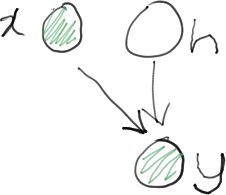
\includegraphics[width=\textwidth,height=4cm,keepaspectratio]{figures/disc.png}
      \begin{itemize}
        \item<2-> $h \in [k] \sim \Mult(\pi)$.
        \item<4-> $y = \beta_h^T x + \epsilon$.
      \end{itemize}
      }};

    \node[style=box] at (6,0) {\obj{%
    \includegraphics<1>[width=\textwidth,height=6cm,keepaspectratio]{figures/mlr-data-2.png}
    \includegraphics<2>[width=\textwidth,height=6cm,keepaspectratio]{figures/mlr-data-3a.png}
    \includegraphics<3>[width=\textwidth,height=6cm,keepaspectratio]{figures/mlr-data-3b.png}
    \includegraphics<4>[width=\textwidth,height=6cm,keepaspectratio]{figures/mlr-data-4a.png}
    \includegraphics<5>[width=\textwidth,height=6cm,keepaspectratio]{figures/mlr-data-4b.png}
    %\includegraphics<6>[width=\textwidth,height=6cm,keepaspectratio]{figures/mlr-data-4c.png}
    \includegraphics<6>[width=\textwidth,height=6cm,keepaspectratio]{figures/mlr-data-5.png}
      }};
  \end{tikzpicture}
\end{frame}

\begin{frame}
  \frametitle{Mixture of Linear Regressions}

  \begin{tikzpicture}
    \node[style=box] (data) at (0,0) {\obj{%
    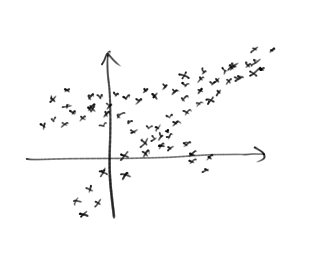
\includegraphics[width=\textwidth,height=6cm,keepaspectratio]{figures/mlr-data-6.png}
      \\{\em Data}
      }};

    % x, y
    \node[style=box] (params) at (7,0) {\objw{4cm}{%
    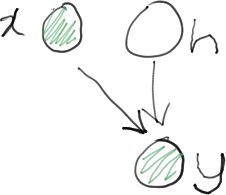
\includegraphics[width=\textwidth,height=4cm,keepaspectratio]{figures/disc.png}
    \\
    {\bf Parameters: $\pi, B$}
    }};

    \draw[->,dashed] (data) -- node[above]{?} (params);


  \end{tikzpicture}
\end{frame}

% \begin{frame}
%   \frametitle{Method of Moments for Generative LVMs.}
% 
%   \begin{tikzpicture}
%     % x, y
%     \node<1->[style=box]  (moments) at (0,0) {\objw{12cm}{%
%       \begin{align*}
%         \underbrace{\E[x]}_{M_1} &= \sum_{h=1}^k \pi_h \beta_h & 
%         \underbrace{\E[x\tp{2}]}_{M_2} &= \sum_{h=1}^k \pi_h \beta_h\tp{2} & 
%         \underbrace{\E[x\tp{3}]}_{M_3} &= \sum_{h=1}^k \pi_h \beta_h\tp{3}. 
%       \end{align*}
%     }};
%     \node<1>[style=box,below=0.1cm of moments] {\objw{12cm}{%
%     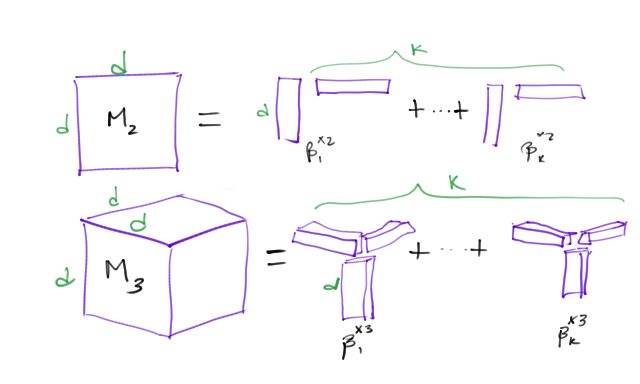
\includegraphics[width=\textwidth,height=6cm,keepaspectratio]{figures/moments.png}
%       }};
%     \node<2->[style=box,below=0.1cm of moments] {\objw{12cm}{%
%       \begin{itemize}
%         \item<2-> {\bf Tensor Power Method} for orthonormal $\beta_h$,
%           \begin{align*}
%             M_3(\beta_h,\beta_h) 
%               &= \sum_{h'=1}^k \pi_{h'} (\beta_{h}^T \beta_{h'})^2 \beta_{h'} \\
%               &= \sum_{h'=1}^k \pi_{h'} \delta_{hh'} \beta_{h'} \\
%               &= \pi_{h'} \beta_{h}.
%           \end{align*}
%         \item<3-> Use $M_2$ to whiten $M_3$.
%       \end{itemize}
%       }};
%   \end{tikzpicture}
% 
%     \note[item]{\bf We can recover the means of a generative LVM by exploiting their symmetric structure.}
%     \note[item]{\begin{align*} M_2 &= \sum_{h=1}^k \pi_h \beta_h\tp{2} & M_3 &= \sum_{h=1}^k \pi_h \beta_h\tp{3}.  \end{align*}}
%       \note[item]{In general, $M_2$ is insufficient to identify the model, because it is invariant to rotations of $B$. }
%       \note[item]{If the $\beta_h$ were orthogonal, then the eigenvectors and eigenvalues of $M_3$ would give us the answer. }
%       \note[item]{In general, we need both $M_2$ and $M_3$. We can use the whitening transformation for $M_2$ to whiten $M_3$ such that it has a orthogonal decomposition.}
%       \note[item]{The robust tensor power method by \cite{AnandkumarHsuGe2012} find stable eigenvectors.}
% \end{frame}

\begin{frame}
  \frametitle{Method of Moments for the Mixture of Linear Regressions.}

  \begin{tikzpicture}
    % x, y
    \node[style=box] at (0,0) {\objw{12cm}{%
        \begin{align*}
          \action<+->{
          y &= \underbrace{\beta_h^T}_{\textrm{random}} x + \epsilon \\
          }
          \action<+->{
            &= \underbrace{\E[\beta_h]^T x}_{\textrm{linear measurement}} + \underbrace{(\beta_h - \E[\beta_h])^T x + \epsilon}_{\textrm{noise}} \\
          }
        \end{align*}
      }};
    %\node[style=box] at (6,0) {\objw{8em}{%
    %  {$y^p$ are linear measurements of the moments of the parameters $M_p$!}
    %  }};
  \end{tikzpicture}

    \note[item]{The powers of the response variables $y^p$ are linear measurements of the moments of the parameters $M_p$!}
    \note[item]{As noted earlier, the first problem we run into is that we can't observe the moments of the parameters $B$ and $\pi$ directly!}
    \note[item]{However, observe that 
    \begin{align}
      y &= \innerp{\beta_h}{x} + \epsilon \\
        &= \innerp{\E[\beta_h]}{x} + \underbrace{{\beta_h - \E[\beta_h]}{x} + \epsilon }_{\textrm{noise}},
    \end{align}
    where $M_1 = \sum_{h=1}^k \pi_h \beta_h$, the mean regression coefficient.}
    \note[item]{We note that while the noise term is dependent on $x$, it has a zero-mean. Thus, we could potentially recover $M_1$ through regression.}
    \note[item]{Similarly, we can cast the remaining two terms as regression problems.}
    \note[item]{An additional fact that we can exploit is that both $M_2$ and $M_3$ are low rank, so we can use low-rank regression to recover estimates $\hat M_2$ and $\hat M_3$ efficiently from data.}
\end{frame}

\begin{frame}
  \frametitle{Method of Moments for the Mixture of Linear Regressions.}

  \begin{tikzpicture}
    % x, y
    \node[style=box] (measurements) at (0,0) {\objw{12cm}{%
        \begin{align*}
          \action<+->{%
            y &= \underbrace{\E[\beta_h]^T \odot x}_{\textrm{linear measurement}} &\quad & + \underbrace{(\beta_h - \E[\beta_h])^T x + \epsilon}_{\textrm{noise}} \\
          }
          \action<+->{%
            y^2 
              &= \E[\beta_h\tp{2}] \odot x\tp{2} &+ \textrm{bias} &+ \textrm{noise} \\
          }
          \action<+->{%
          y^3 &= \E[\beta_h\tp{2}] \odot x\tp{3} &+ \textrm{bias} &+ \textrm{noise} \\
          }
        \end{align*}

        \uncover<4->{%
          We can use regression to recover $M_p$ from linear measurements.\\
          }
      }};
  \end{tikzpicture}
\end{frame}

\begin{frame}
  \frametitle{Method of Moments for the Mixture of Linear Regressions.}

  \begin{tikzpicture}
    % x, y
    \node[style=box] (measurements) at (0,0) {\objw{12cm}{%
      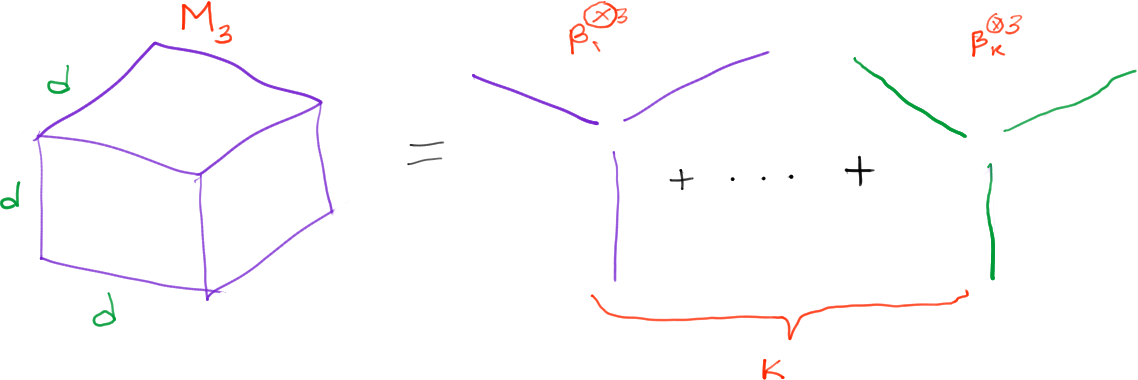
\includegraphics[width=\textwidth,height=6cm,keepaspectratio]{figures/tensor.png}
      }};
    \node<2->[style=box,below=0.1cm of measurements] {\objw{12cm}{%
      We can use low-rank regression techniques [Negabhan \& Wainwright 2009; Tomioka 2011].
      \begin{align*}
        \hat\E[\beta_h\tp{2}] &= \arg\min_{M} \left(y^2 - M] \odot x\tp{2}\right)^2_{(x,y)\in\mathcal{D}} + \|M\|_{*} \\
        \|M\|_{*} &= \sum_i \sigma_i(M).
      \end{align*}
      }};
  \end{tikzpicture}
\end{frame}

% \begin{frame}
%   \frametitle{Method of Moments for the Mixture of Linear Regressions.}
% 
%   \begin{tikzpicture}
%     % x, y
%     \node[style=box] (note) at (0,0) {\objw{12cm}{%
%       {$y^p$ are linear measurements of the moments of the parameters $M_p$!}
%       }};
%     \node[style=box,below=0.1cm of note] {\objw{12cm}{%
%       \includegraphics<1>[width=\textwidth,height=8cm,keepaspectratio]{figures/regression-1.png}
%       \includegraphics<2>[width=\textwidth,height=8cm,keepaspectratio]{figures/regression-2.png}
%       \includegraphics<3>[width=\textwidth,height=8cm,keepaspectratio]{figures/regression-3.png}
%       }};
%   \end{tikzpicture}
% \end{frame}

\begin{frame}
  \frametitle{Overview: Spectral Experts}

  \begin{tikzpicture}
    % x, y
    \node[style=box] at (0,0) {\objw{12cm}{%
      \includegraphics<1>[width=\textwidth,height=8cm,keepaspectratio]{figures/err-1.png}
      }};
  \end{tikzpicture}
\end{frame}

\begin{frame}
  \frametitle{Perturbation Analysis}

  \begin{tikzpicture}
    % x, y
    \node[style=box] at (0,0) {\objw{12cm}{%
      \includegraphics<1>[width=\textwidth,height=8cm,keepaspectratio]{figures/err-1.png}
      %\includegraphics<2>[width=\textwidth,height=8cm,keepaspectratio]{figures/err-2.png}
      \includegraphics<2>[width=\textwidth,height=8cm,keepaspectratio]{figures/err-3.png}
      %\includegraphics<4>[width=\textwidth,height=8cm,keepaspectratio]{figures/err-4.png}
      \includegraphics<3>[width=\textwidth,height=8cm,keepaspectratio]{figures/err-5.png}
      }};
  \end{tikzpicture}

  \note[item]{The algorithm is consistent, and requires $O(?)$ samples.}
  \note[item]{The rate of convergence for the spectral experts algorithm to the true parameters breaks into two parts; the rates for learning the moments, which feeds into the rates for learning the parameters.}
  \note[item]{For low rank regression, we have the following bound on recovery by (Tomioka2011); $$ \| \hat M_p - M_p \|_F \le \frac{32 \lambda^{(p)}_n \sqrt{k}}{\kappa(\opX_p)}, $$ where $\kappa(\opX_p)$ is the (restricted) strong convexity constant, and $\lambda^{(p)} > \|\opX^*_p(\eta)\|$.}
  \note[item]{Because we assume our noise is bounded, it is easy to show that the error concentrates.}
  \note[item]{In the tensor recovery case, we will need to whiten $M_3$ before applying the tensor decomposition and unwhiten it afterwards; this modifies the error bounds slightly.}
\end{frame}

\begin{frame}
  \frametitle{Experimental Insights}

  \begin{tikzpicture}
    % x, y
    \node<-4> (em) at (-3,-0.5) {%
      \includegraphics<1>[width=\textwidth,height=5cm,keepaspectratio]{figures/1-8-3.png}
      \includegraphics<2->[width=\textwidth,height=5cm,keepaspectratio]{figures/1-8-3-em.png}
      };
    % x, y
    \node<-4> at (3,-0.5) {%
      \includegraphics<3>[width=\textwidth,height=5cm,keepaspectratio]{figures/1-8-3-spec.png}
      \includegraphics<4->[width=\textwidth,height=5cm,keepaspectratio]{figures/1-8-3-specm.png}
      };
    \node<5-> at (0,-0.5) {%
      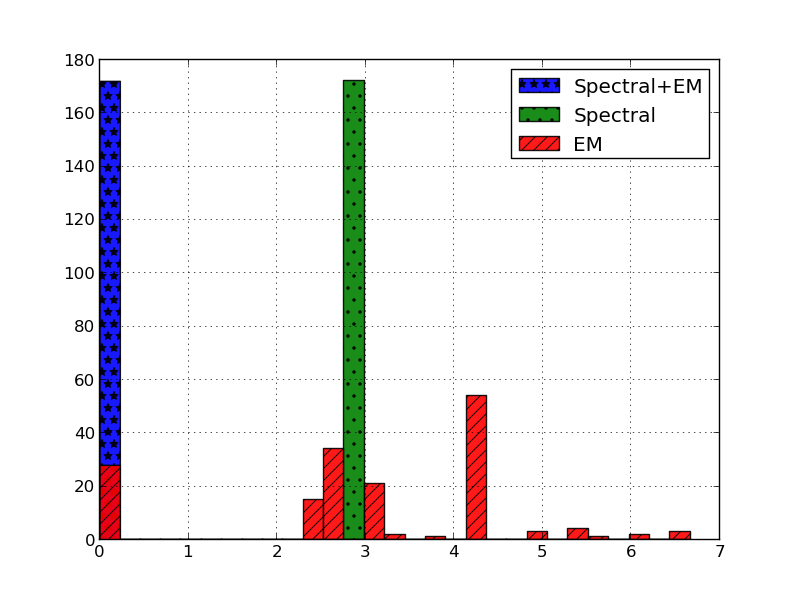
\includegraphics[width=\textwidth,height=5cm,keepaspectratio]{figures/hist.png}
    };

    \node[above=0.1 cm of em] {%
    $y = \underbrace{t + t^4 + t^7}_{x} + \epsilon$
    };

%      \begin{small}
%  \begin{tabular}{ r r r c c c }
%\hline
%$b$ & $d$ & $k$ & Spectral & EM & Spectral + EM \\
%\hline
%  1 & 4 & 2 & 2.45 $\pm$ 3.68 & 0.28 $\pm$ 0.82 & {\bf 0.17 $\pm$ 0.57} \\
%  2 & 5 & 2 & 1.38 $\pm$ 0.84 & {\bf 0.00 $\pm$ 0.00} & {\bf 0.00 $\pm$ 0.00} \\
%  2 & 5 & 3 & 2.92 $\pm$ 1.71 & 0.43 $\pm$ 1.07 & {\bf 0.31 $\pm$ 1.02} \\
%  2 & 6 & 2 & 2.33 $\pm$ 0.67 & 0.63 $\pm$ 1.29 & {\bf 0.01 $\pm$ 0.01} \\
%\hline
%\end{tabular}
%      \end{small}
%    }};
  \end{tikzpicture}

  \note[item]{Stable!}
    \note[item]{Spectral Experts provides a good initialization to EM.}
    \note[item]{We simulated the performance of spectral experts and compared it to EM.}
    \note[item]{In a non-trivial number of cases, EM did not converge to the right parameters and got stuck in local optima.}
    \note[item]{The parameters estimated by the spectral method were not very good even with $O(10^5)$ samples.}
    \note[item]{However, EM initialized with these parameters did extremely well.}
\note[item]{This finding that spectral methods should be a good initialization for EM is not surprising.}
\note[item]{%
  \begin{itemize}
    \item The biggest sell for spectral methods is that they give a global guarantee on where the parameters are.
    \item The parameters might not be at the global optima, but will hopefully lie in the potential well around it.
    \item EM will then converge to the global optima.
  \end{itemize}
  }
\end{frame}

\begin{frame}
  \frametitle{Experimental Insights}

  \begin{tikzpicture}
    \node[style=box] at (0,-1.5) {\objw{12cm}{%
      \includegraphics<1>[width=\textwidth,height=6cm,keepaspectratio]{figures/likelihood-mom.png}
      \includegraphics<2>[width=\textwidth,height=6cm,keepaspectratio]{figures/likelihood-mom-em1.png}
      \includegraphics<3>[width=\textwidth,height=6cm,keepaspectratio]{figures/likelihood-mom-em2.png}
        \hfill{\em expected log-likelihood}
      }};
  \end{tikzpicture}

\end{frame}


\begin{frame}
  \frametitle{Conclusions}
  \begin{itemize}
    \item {\bf Consistent estimator} for the mixture of linear regressions with {\bf polynomial sample and computational complexity}.
    \item<2-> Derive conditional moments using regression.
    \item<3-> Method of moment estimates can be a good initialization for EM.
  \end{itemize}
\end{frame}

\begin{frame}
  \frametitle{}
    Thank you.
\end{frame}

\end{document}

% TikZ
%\begin{tikzpicture}
%  \node (img1) at (0,0) {\includegraphics[height=0.6\textheight,width=0.4\linewidth,keepaspectratio]{}};
%\end{tikzpicture}

% Notes 
% \note[item]{}

% 2-column
% \begin{columns}
%   \begin{column}{0.48\textwidth}
%     \begin{itemize}
%         \item
%     \end{itemize}
%   \end{column}
%   \hfill
%   \begin{column}{0.48\textwidth}
%     \begin{itemize}
%         \item
%     \end{itemize}
%   \end{column}
% \end{columns}

% TikZ
%\begin{tikzpicture}
%  \node (img1) at (0,0) {\includegraphics[height=0.6\textheight,width=0.4\linewidth,keepaspectratio]{}};
%\end{tikzpicture}

% Notes 
% \note[item]{}

% 2-column
% \begin{columns}
%   \begin{column}{0.48\textwidth}
%     \begin{itemize}
%         \item
%     \end{itemize}
%   \end{column}
%   \hfill
%   \begin{column}{0.48\textwidth}
%     \begin{itemize}
%         \item
%     \end{itemize}
%   \end{column}
% \end{columns}

